\section{UDP vs. basic IP}

\begin{frame}{UDP vs. basic IP}{Use reinforced libraries!}
	\begin{alertblock}{High performance parallel programming is hard stuff!}
		\begin{itemize}
		  \item Patterns like thread-per-connection are very inefficient!
		  \item Patterns like proactor (thread per core) are complex to implement!
		\end{itemize}
	\end{alertblock}

	
	\begin{block}{Don't reinvent the wheel! Use UDP/TCP via popular libraries.}
		Libs like boost::asio make live easier and ``boost'' the performance.
		\\
		Using basic IP will make it impossible to use all the functionality of those
		libraries.
	\end{block}
	
	\begin{ergo}
		As long as low latency is not of high importance, I would stick to reinforced
		internet standards like UDP and TCP and implement those with external
		libraries like boost::asio!
	\end{ergo}
\end{frame}

\section{Endianess}

\begin{frame}[fragile]
\frametitle{Little endian simplifies software}
\framesubtitle{But performance costs of ntohl only one clock ($\approx0.33 ns$)}
	\begin{figure}[htp]
		\begin{center}
		  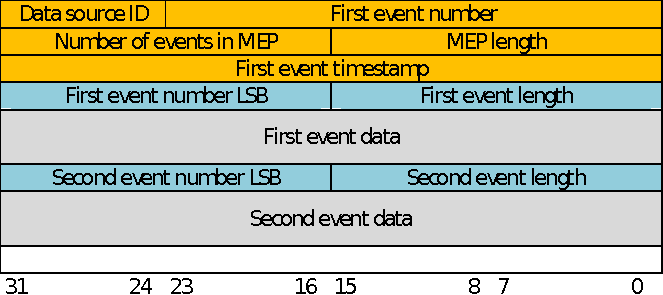
\includegraphics[width=6cm]{mep}
		\end{center}
	\end{figure}
\begin{lstlisting}[frame=trBL,caption={}]{hallowelt}
socket.receive(data);
// No ntohl needed:
memcpy(&firstEventNum,&data[0], 3);
memcpy(&sourceID,&data[3], 1);
memcpy(&mepLength,&data[4], 2);
memcpy(&eventCount,&data[6], 2);
memcpy(&firstTimestamp,&data[8], 4); 
\end{lstlisting}

\end{frame}


\section{Backup:}

\begin{frame}{}
	\begin{center}
		\textbf{Backup}
	\end{center} 
\end{frame}


\section{Monitoring}


\begin{frame}{GWT: An application-like website}{Monitoring via your web browser}
	Every L1/L2 machine writes it's statistics data to one central MySQL server.
	This data will be summarized via GWT.
	\begin{block}{\textbf{G}oogle \textbf{W}eb \textbf{T}oolkit }
		\begin{itemize}
		  \item Mainly a Java to JavaScript compiler
		  \item Duplex communication between client and server possible
		  \item No HTML, PHP/Ruby, Javascript, CSS knowledge needed!
		  \item Only Java (and SQL)!!!
		\end{itemize}
		\begin{ergo}
			Feels like a locale application without X11-tunneling, program download...
			\textbf{just a standard web browser needed}
		\end{ergo}
	\end{block}
\end{frame}


\begin{frame}{What should be displayed}
	\begin{block}{Level 0}
		\begin{itemize}
		  \item Trigger rate and distribution
		  \item MEP rate to L1
		  \item Data rate to L1
		\end{itemize}	
	\end{block}
	
		\begin{block}{Level 1/2}
		\begin{itemize}
		  \item Packet loss rate
		  \item Broken event rate
		  \item Processing time of each level
		  \item Load (Memory, CPU)
		  \item Trigger rates and distribution (L1 \& L2)
		  \item Data rates to persistent memories
		\end{itemize}
	\end{block}
\end{frame}

\begin{frame}{Coincidence with bursts}
	I'd like to show most of the data in relation to the burst number.
	
	\begin{ergo}
		How do I get the burst number corresponding to the event numbers?!
	\end{ergo}
	
	\vspace{1cm}
	If L0TP is a PC I would let it write this data to the ``Burst'' table of
	my monitoring database (*\_ID are foreign keys):
	\begin{table}
		\begin{tabular}{ccc}
			ID	&	FirstEvent\_ID	&	LastEvent\_ID \\
		\end{tabular}
	\end{table} 
\end{frame}








\section{boost::asio}
\lstloadlanguages{C++}
\lstset{language=C++, frameround=fttt, breaklines=true, tabsize=2,
keywordstyle=\color{blue},labelstyle=\tiny, labelstep=5, firstlabel=1, labelsep=5pt, numbers=left}

\begin{frame}{boost::asio}
	\begin{block}{Why I want to use boost::asio}
		\begin{itemize}
		  \item Less code
		  \item More readable code
		  \item Proactor design pattern
		  \item Don't want to reinvent the wheel!
		\end{itemize}
	\end{block}
	\begin{exampleblock}{Proactor design pattern (Think asynchronous!)}
		\begin{itemize}
		  \item Almost no synchronization needed
		  \item Thread per core, not per connection
		  \item Less context switching $\Rightarrow$ better performance
		\end{itemize}
	\end{exampleblock}
\end{frame}

\begin{frame}[fragile]
\frametitle{Sample program}
\framesubtitle{Proactor design pattern: Initiator}
\begin{lstlisting}[frame=trBL,caption={}]{hallowelt}
boost::asio::io_service io_service;
udp::socket socket_(io_service, udp::endpoint(udp::v4(), port_));
socket_.async_receive(boost::asio::buffer(buffer_),boost::bind(&udp_server::handle_receive,this, boost::asio::placeholders::bytes_transferred)); 
for (int i=0; i < 24; i++) 
		boost::thread t(boost::bind(&boost::asio::io_service::run,&io_service));
\end{lstlisting}
\end{frame}

\begin{frame}[fragile]
\frametitle{Sample program}
\framesubtitle{Proactor design pattern: Completion Handler}

\begin{lstlisting}[frame=trBL,caption={}]{hallowelt}
handle_receive(const size_t& bytesReceived) {
    char* data = buffer_;
    buffer_ = malloc(9000);
    // Let enother thread read next pack
    socket_.async_receive(boost::...
    
    DO SOME WORK WITH data HERE!!!
}
\end{lstlisting}
\end{frame}
